\section{Off-peak Phase Selection}
\seclabel{peak_definition}

We first developed a systematic, model-independent, and
computationally-efficient method to define the off-peak interval of a
pulsar light curve.

We begin by deconstructing the light curve into simple Bayesian Blocks
using the algorithm described in \citet{jackson_2005a_algorithm-optimal}
and \citet{scargle_2013a_studies-astronomical}.  We could not apply the
Bayesian Block algorithm to the weighted-counts light curves because
they do not follow Poisson statistics, required by the algorithm.
We therefore use an unweighted-counts light curve in which the angular
radius and minimum energy selection have been varied to maximize the
H-test statistic.  To produce Bayesian Blocks on a periodic light curve,
we extend the data over three rotations, by copying and shifting the
observed phases to cover the phase range from $-$1 to 2.  We do, however,
define the final blocks to be between phases 0 and 1.  To avoid potential
contamination from the trailing or leading edges of the peaks, we reduce
the extent of the block by 10\% on either side, referenced to the center
of the block.

There is one free parameter in the Bayesian Block algorithm called ncp$\rm
_{prior}$ which modifies the probability that the algorithm will divide
a block into smaller intervals.  We found that, in most cases, setting
ncp$\rm _{prior}=8$ protects against the Bayesian Block decomposition
containing unphysically small blocks.  For a few marginally-detected
pulsars, the algorithm failed to find more than one block and we had to
decrease ncp$\rm _{prior}$ until the algorithm found a variable light
curve. Finally, for a few pulsars the Bayesian-block decomposition of the
light curves failed to model weak peaks found by the light-curve fitting
method presented in \citep{abdo_2013a_second-fermi} or extended too far
into the other peaks. For these pulsars, we conservatively shrink the
off-peak region.

For some pulsars, the observed light curve has two well-separated peaks
with no significant bridge emission, which leads to two well-defined
off-peak intervals.  We account for this possibility by finding the
second-lowest Bayesian block and accepting it as a second off-peak
interval if the emission is consistent with that in the lowest block
(at the 99\% confidence level) and if the extent of the second block is
at least half that of the first block.

\figref{off_peak_select} shows the energy-and-radius optimized light
curves, the Bayesian block decompositions, and the off-peak intervals for
six pulsars.  \citep{abdo_2013a_second-fermi} overlay off-peak intervals
over the weighted light curves of several pulsars.  The off-peak intervals
for all pulsars are given in \citep{abdo_2013a_second-fermi}.

\begin{figure}
  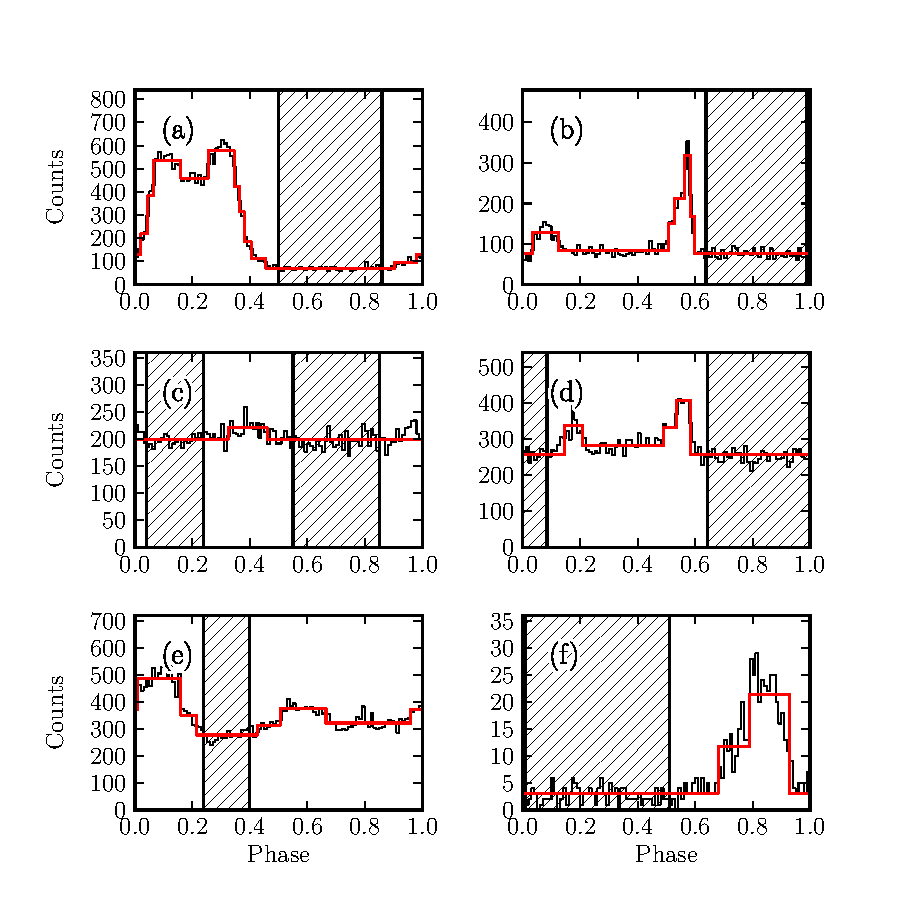
\includegraphics{chapters/offpeak/figures/off_peak_phase_color.pdf}
  \caption{The energy-and-radius optimized light curve, Bayesian
  block decomposition of the light curve, and off-peak interval for
  (a) PSR J0007+7303, (b) PSR J0205+6449, (c) PSR J1410$-$6132, (d) PSR
  J1747$-$2958, (e) PSR J2021+4026, and (f) PSR J2124$-$3358.  The black
  histograms represent the light curves, the gray lines (colored red in
  the electronic version) represent the Bayesian block decompositions of
  the pulsar light curves, and the hatched areas represent the off-peak
  intervals selected by this method.}
  \figlabel{off_peak_select}
\end{figure}

